\chapter{Photochemistry}
With the arsenal of methods discussed in Chapters \ref{chap:meth} and \ref{chap:emb}, we are in a position to model some photochemical systems in the excited state. This chapter outlines the theory behind photochemistry in the vacuum and aggregate phases so that we can better understand the phenomena we are trying to model.

\section{Absorption}
\subsection{Principles of Photochemistry}
Light-induced chemical processes follow two fundamental laws:\cite{Persico2018}
\begin{itemize}
    \item \textbf{Grotthuss–Draper Law}: Only light which is absorbed by the chemical system can produce change.
    \item \textbf{Stark–Einstein Law}: The energy of each absorbed photon corresponds to the energy difference between the initial and newly excited states of the system.
\end{itemize}
The combination of these laws implies that in order for a photochemical process to occur, the incident photons to the chromophore need to be of an energy matching an allowed electronic transition. This gain in energy takes the wavefunction from its original ground state to a new, excited state one.

In the BO approximation, the energy of the molecular wavefunction depends parametrically on the nuclear coordinates. This implies that for a given electronic excitation state, there is a continuous hyperdimensional landscape which maps a set of nuclear coordinates to a potential energy. Such Potential Energy Surfaces (PESs) are represented in Figure \ref{fig:pes_example}, displaying different excited state mechanisms (see later subsections).

\begin{figure}
\centering
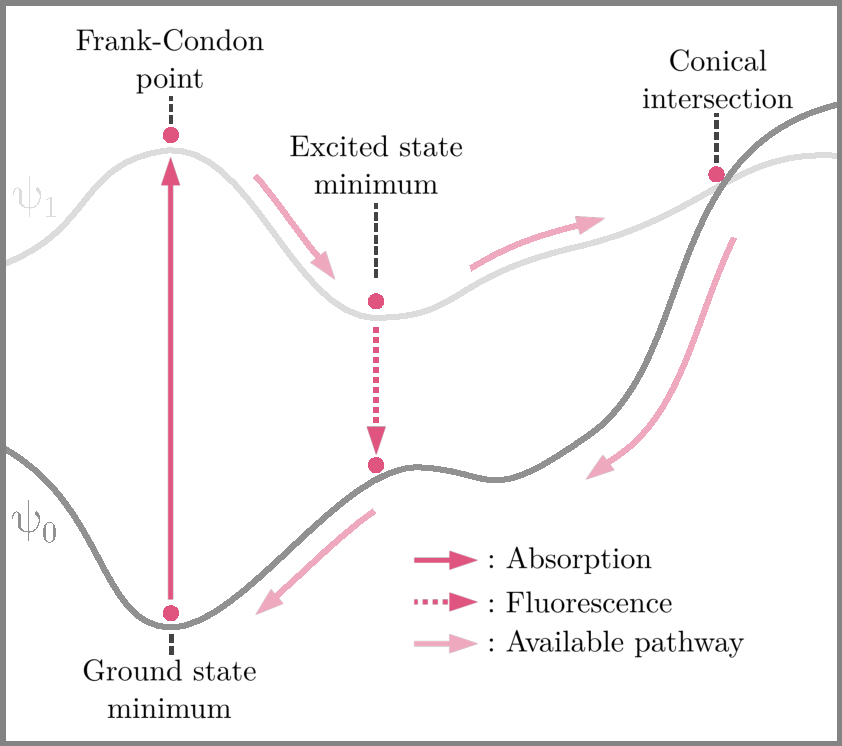
\includegraphics[width=10cm]{Chapters/4Photochem/PES.pdf}
\caption{Example of a potential energy surface demonstrating either a radiative decay \textit{via} fluorescence, or a nonradiative decay \textit{via} funnelling through a conical intersection.}
\label{fig:pes_example}
\end{figure}

First, bringing our attention to the absorption process, we can see how the difference in energy between two potential energy surfaces at a fixed ground state geometry would correspond to the energy of one photon. Even considering all of the possible excitations present in the full CI expansion of Equation \ref{eq:fullci}, electronically excited states only occupy discrete levels of energy, in this limited picture. In reality, molecular and crystalline systems absorb as continuous spectra across the electromagnetic range, as shown in Figure \ref{fig:hpp_abs} for the 2-hydroxyphenyl)propenone single crystal. This material holds promise for solid state luminescent applications such as lasers or OLEDs.\cite{Tang2016a}

\begin{figure}
\centering
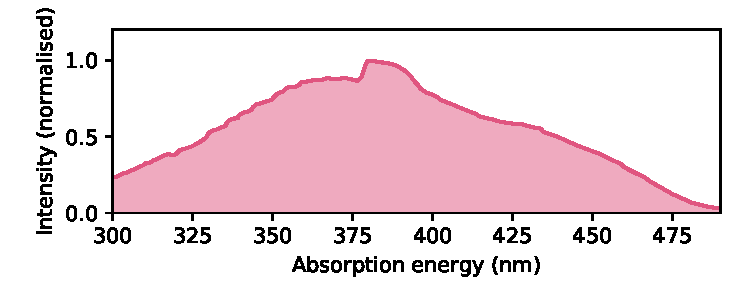
\includegraphics[width=10cm]{Chapters/4Photochem/hpp_abs.pdf}
\caption{Absorption spectrum of (2-hydroxyphenyl)propenone (HPP) in single crystal form.\cite{Tang2016a}}
\label{fig:hpp_abs}
\end{figure}

Several effects contribute to the broadening and mixing of the excitation energies, shaping this absorption spectrum.

\subsection{Oscillator Strength}
\label{sec:osci}
First, we will investigate what the probability is of photons being absorbed for a given transition.

To answer this, we begin by examining the transition dipole moment (TDM) between an initial state $i$ and final state $j$:
\begin{equation}
    (\bm{T}_{ij})_x = \int \psi^*_j(\bm{r}) \hat{x} \psi_i(\bm{r}) d\bm{r}
    \label{eq:tdm}
\end{equation}
Where $\psi_n(\bm{r})$ is the wavefunction of state $n$. This equation gives the $x$ component of the total vector TDM, $\bm{T}_{ij}$. The probability of transition from one quantum state to another is worked out from the quantum eleoctrodynamical treatment of spontaneous emission. It is
proportional to the square of the TDM, and to the energy gap between the states:\cite{Hilborn1982}
\begin{equation}
    f_{ij} \propto (E_j - E_i) \abs{\bm{T}_{ij}}^2
\end{equation}
Where $E_n$ is the energy of state $n$, and $f_{ij}$ is called the \textit{oscillator strength} of the transition $i \rightarrow j$. The oscillator strength can therefore serve as a measure of the likelihood of population of different excited states, depending on the frequency of the incident light.

\subsection{Natural Linewidth}

For a given molecule, we therefore have several energy levels at which photons can be absorbed, with different probabilities. Additionally, we should consider the energy-time form of the uncertainty principle:
\begin{equation}
    \Delta E \Delta t \geq \frac{\hbar}{2}
\end{equation}
Which imposes a minimum on the product between the uncertainty in the excited state energy $\Delta E$ and the uncertainty in its lifetime $\Delta t$. There is therefore a so called \textit{natural linewidth} which ensures that incident photons do not need to match the energy difference between states at infinite precision.


\subsection{Role of Vibrations}

Note that the wavefunctions in Equation \ref{eq:tdm} have both an electronic an a nuclear part. Working under the BO approximation, these parts can be factorised, and the transition dipole moment ends up accounting for both the change in dipole from the transition of the electron cloud, and the overlap between the nuclear vibrational states. Labelling the different potential states involved in a transition as $\psi_{n,\nu_m}$, for the $m$th electronic excitation and $M$th vibrational substate, we end up with a large amount of possible combinations, depicted schematically in Figure \ref{fig:manifold}.

\begin{figure}
\centering
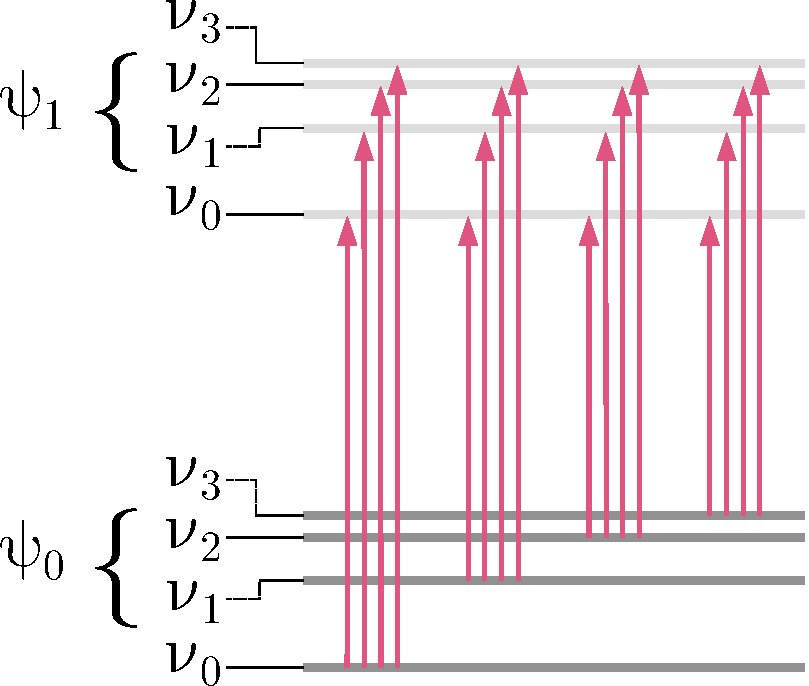
\includegraphics[width=10cm]{Chapters/4Photochem/jablo.pdf}
\caption{Diagram showing the manifold of transitions between two electronic states, each with four vibrational substates. The electronic wavefunctions are denoted $\psi_n$ and the vibrational states $\nu_m$.}
\label{fig:manifold}
\end{figure}

Moreover, for periodic materials, we consider lattice vibrations rather than molecular ones, and bands of energy rather than discrete levels. This further contributes to the continuity of the spectrum in Figure \ref{fig:hpp_abs}

\section{Emission}

We now return to Figure \ref{fig:pes_example} to understand what can happen to the molecule after excitation. If the molecular system is at rest at the time of absorption, its nuclear coordinates will be at the point of lowest energy, the ground state geometry. The corresponding excited state at the same geometry is reached after absorption, and is referred to as the \textit{Frank-Condon point} (FC). Since the FC geometry is unlikely to be a minimum of the excited state potential energy surface, the molecule will have enough energy to travel downhill (or through tunnelling, or extra vibrational energy) to new nuclear configurations.

\subsection{Fluorescence}
When the excited state reaches a minimum geometry, the molecule naturally oscillates around this minimum. However excited states are by definition metastable, and therefore the energy difference between ground and excited state must be released in some way. Such transitions from states of same multiplicity are called \textit{fluorescence}. When a molecule fluoresces, it emits a photon of the frequency corresponding to the difference in energy between excited and ground state.

The lifetime of this process is dependent on the overlap of the wavefunctions of initial and final state (see Section \ref{sec:osci}) and the relative populations of the two states within the chemical system. The result is usually lifetimes of the order of nanoseconds.

\subsection{Phosphorescence}
In certain cases, as a part of the excited state mechanism, the wavefunction may enter a state of different multiplicity than the ground state. In this case, after reaching the excited state minimum, the transition between states is classically forbidden due to the spin flip involved. The process may still occur, but the lifetime of phosphorescence can reach minutes or hours.


\section{Nonradiative Decay}
Electronic wavefunctions can also decay from the excited to the ground state nonradiatively. Understanding how to limit this behaviour is essential in designing efficient luminescent materials.

\subsection{Vibrational Internal Conversion}
\label{sec:fgr}

Fermi's Golden Rule (FGR) gives an expression for the rate of transfer between quantum states under small perturbations.\cite{dirac1927} The nonradiative transition between separate excited state of the same spin multiplicity in the adiabatic regime is called internal conversion. Derived from perturbation theory on the TDSE, FGR states:
\begin{equation}
    k_{\text{IC}}^{\text{Fermi}} = \frac{2\pi}{\hbar} \sum_{\nu_i,\nu_f} P_{i\nu_i}(T) \abs{\sum_k \bra{\Psi_{f,\nu_f}}\hat{P}_k\ket{\Psi_{i,\nu_i}}}^2 \delta(E_{i\nu_i} - E_{f\nu_f})
    \label{eq:fermiprime}
\end{equation}

Where $P_{i\nu_i}(T)$ is the Boltzmann distribution at temperature $T$ of the vibrational manifold at the initial electronic state, $\Psi_{n,\nu_n}$ is the wavefunction at electronically excited state $n$ and vibrational state $\nu_n$, and $\hat{P}_k$ are the nuclear momentum operators for the $k$-th normal mode of vibration.

In the BO approximation, we can separate the wavefunction $\ket{\Psi_{i\nu_i}}=\ket{\Phi_i \Theta_{i\nu_i}}$ into a product $\ket{\Psi_{i\nu_i}}=\ket{\Phi_i} \ket{\Theta_{i\nu_i}}$, where $\Phi_i$ is the electronic wavefunction and $\Theta_{i\nu_i}$ is the vibrational wavefunction.

This allows us to rearrange the internal conversion rate as follows:\cite{Niu2010,Peng2016c}
\begin{equation}
    k_{\text{IC}}^{\text{Fermi}} = \frac{2\pi}{\hbar} \sum_{\nu_i,\nu_f} P_{i\nu_i}(T) \abs{\sum_k \bra{\Phi_f}\hat{P}_k\ket{\Phi_i} \bra{\Theta_{f\nu_f}}\hat{P}_k\ket{\Theta_{i\nu_i}}}^2 \delta(E_{i\nu_i} - E_{f\nu_f})
    \label{eq:fermi}
\end{equation}

All else being fixed, this allows us to express the rate of internal conversion in terms of the overlap between vibrational wavefunctions, which can be rationalised as the energy barrier between PESs being overcome by thermal vibrations.

Under FGR, the transition occurs between degenerate vibrational states rather than necessarily degenerate electronic ones. Because of this, the numerical methods for solving Equation \ref{eq:fermi} use approximations for the nuclear motion of the molecule, such as a harmonic potential. This potentially leaves out points of degeneracy far from excited state minima.

\subsection{Conical Intersections}
\label{sec:conicals_sec}
In certain scenarios, however, the excited and ground electronic potential energy surfaces are prone to meeting, as is shown in the rightmost phenomenon of Figure \ref{fig:pes_example}. In this case, the time-dependent SE has two degenerate solutions. Additionally, the coupling between excited and ground states also has critical points, where the adiabatic separation between them breaks down. The points which combine these two conditions allow for the funnelling of the wavefunction from the excited to the ground state without emission at any point.

We can inspect these exceptional cases by enclosing the TISE in wavefunctions in the Born-Huang representation:
\begin{equation}
    \ket{\Psi} = \sum_i^\infty \ket{\Phi_i} \ket{\Theta_i}
    \label{eq:bornhuang}
\end{equation}
Where we have separated the electronic wavefunction $\Phi$ from the nuclear one $\Theta$ and labeled the excited state $i$.

The result is that sufficient condition for this particular degeneracy to occur between states $i$ and $j$, is the following:
\begin{equation}
    \bm{v}_{ij} = \frac{\bra{\Phi_i} \frac{\partial \hat{H}^{\text{el}}}{\partial \bm{R}} \ket{\Phi_j} }{E_j-E_i} \rightarrow \infty
\end{equation}

\begin{equation}
    \bm{g}_{ij} = \frac{\partial}{\partial \bm{R}} \left(\bra{\Phi_i} \hat{H}^{\text{el}} \ket{\Phi_i} - \bra{\Phi_j} \hat{H}^{\text{el}} \ket{\Phi_j}\right) = 0
\end{equation}

Where $\Phi_n$ is the electronic wavefunction of state $n$, $\hat{H}^{\text{el}}$ is the electronic Hamiltonian, $E_n$ is the energy of state $n$, and $\bm{R}$ are the nuclear coordinates. $\bm{v}_{ij}$ is called the nonadiabatic coupling vector and $\bm{g}_{ij}$ is the derivative coupling vector.\cite{Mead1982}

The intersections are \textit{conical} because they are determined by two coordinates in hyperspace. They should be understood as a multidimensional seam in the potential energy surfaces.\cite{Yarkony1998} This leads us to consider the point of lowest energy along that seam with special interest. The Minimal Energy Conical Intersection (MECI), is an important geometry to characterise, since energy relative to that of the FC geometry dictates its accessibility, and thus the availability of a nonradiative decay channel.

We should clarify the distinction between this decay and the internal conversion through thermal vibrations. The former involves a seam of electronically degenerate states, attainable through thermal motion. The latter directly has to do with the overlap of vibrational wavefunctions, and provides a probability of transition. Both decays can be attained through vibrations, though they are distinct processes which can collaborate or not. Conical intersection decay is the dominant one in the strongly nonadiabatic regions of the PES and \textit{vice versa} elsewhere.\cite{Escudero2019}

\section{Excited States in Aggregates}
\subsection{Excitons}
In molecular aggregates, it is possible for the excited state process to delocalise over several molecules. A collection of thus correlated excited states is called an exciton, when speaking at the molecular scale. As a semantic aside, when considering a lattice, excitons usually refer to an electron-hole pair; however, for small groups of molecules, this charge separation is usually much less distinct, and we call exciton what a spectroscopist might call an "exciplex". Our convention is in line with the language used in the field of molecular photochemistry at the aggregate scale.\cite{Arag2015,Fornari2017,Jurinovich2018}

For clarity of explanation, we will consider the case of two molecules, but know that much of what is discussed is generalisable to the trimer, tetramer, and so on.

Two neighbouring molecules are said to be excitonically coupled if their excited states in isolation are different to those as a dimer. We can quantify this exciton coupling by writing the Hamiltonian of the molecular system in the diabatic basis:
\begin{gather}
    H^{\text{D}} = 
    \begin{pmatrix}
    E^{\text{D}}_1 & J\\
    J & E^{\text{D}}_2
    \end{pmatrix}
\end{gather}
where $E^{\text{D}}_n$ is the diabatic energy of state $n$ and $J$ is the exciton coupling.

\subsection{Kasha's Model}
Obtaining the above Hamiltonian matrix is not a trivial effort, therefore a common approximation is employed to characterise the excitonic states is to reduce each molecule to a point dipole and investigate their electrostatic interaction upon transition. In this case, the relative arrangement of the point dipoles determines the exciton coupling. The expression for the exciton coupling between two molecules $i$ and $j$ can be derived by the Coulomb energy of two point dipoles. It is, in atomic units:\cite{Kasha1965}
\begin{equation}
    J_{ij}=\frac{1}{r_{ij}^3}\left(\bm{\mu}_i \cdot \bm{\mu}_j - 3 \frac{(\bm{\mu}_i \cdot \bm{r}_ij)(\cdot \bm{r}_ij \cdot \bm{\mu}_j)}{|\bm{r}_{ij}|^2}\right)
    \label{eq:kashaequation}
\end{equation}
Where $\bm{\mu}_i$ and $\bm{\mu}_j$ are the transition dipole moments for each molecule and $\bm{r}_{ij}$ is the distance between their centroids. This approximation, known as Kasha's exciton model, is used to rationalise the blue or red shifting of the excitation of molecules in aggregate due to collective excitation.

The exciton coupling causes a splitting of the multi-molecular excited state, thereby selecting the ordering between the symmetric and antisymmetric combination, and the allowed same-symmetry radiative decay transition.\cite{Gierschner2016} Dimers with a negative coupling have the $\frac{\ket{i}+\ket{j}}{\sqrt{2}}$ wavefunction lower in energy than the $\frac{\ket{i}-\ket{j}}{\sqrt{2}}$ wavefunction, and are denoted J aggregates. The opposite is the case for H aggregates.

Due to the dot products in Equation \ref{eq:kashaequation}, the sign of $J_{ij}$, and therefore the classification of the dimer, solely hinges upon the angle between transition dipole moments, and the vector between the monomer's centroids. The transition occurs at an angle of 54.7\degree{}.

Following Kasha's rule, decay to the ground state overwhelmingly happens from the lowest energy excited state. Therefore, for H aggregates, radiative decay is quenched and blue shifted, while for J aggregates, it is red shifted.

\subsection{Types of Exciton}

Of course, in reality, the electron density of the two monomers does not behave like a static point dipole. Beyond the missing short-range interactions and the higher resolution of the Coulomb potential, one should also take into account the reorganisation of the density inter- and intramolecularly.\cite{Fornari2017}

Indeed three extreme scenarios are possible, represented on Figure \ref{fig:exciton_ex}. Upon excitation, the electron density of each molecule can reorganise within and between them. The exciton is then said to be delocalised. In a different case, the reorganisation could be confined to only one molecule, making the exciton localised, occasionally called a Frenkel exciton. Finally, the electron density can migrate from one molecule to another, producing a charge transfer (CT) state.\cite{Hestand2018}

\begin{figure}
\centering
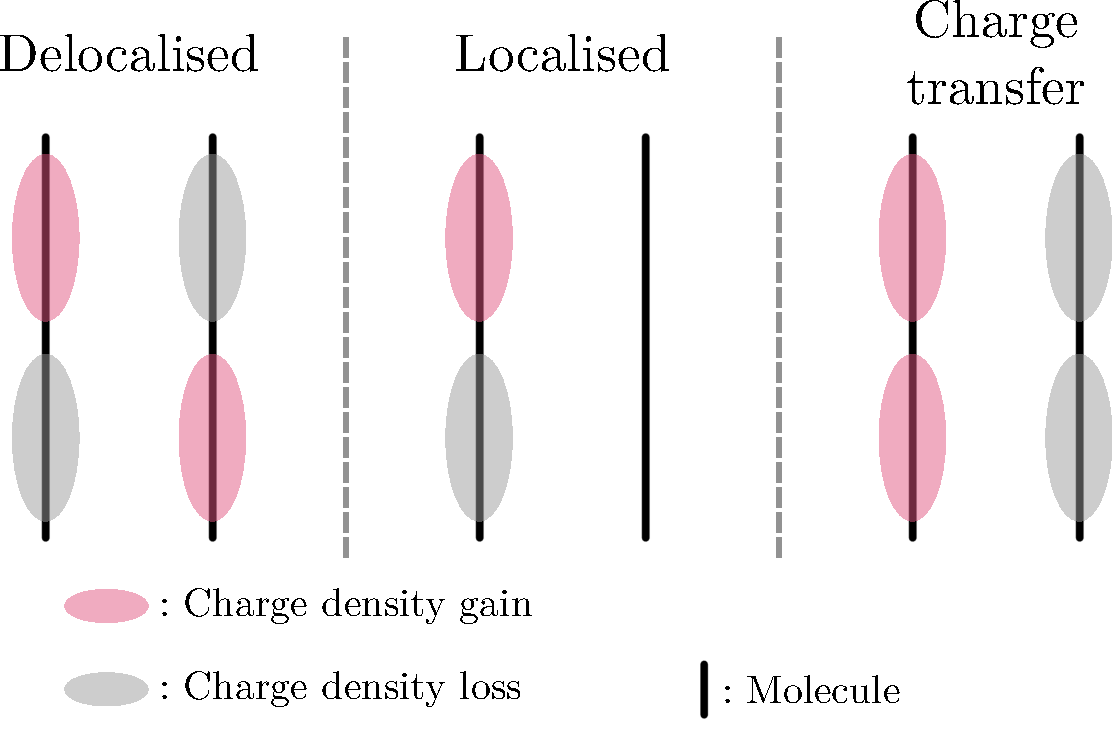
\includegraphics[width=8cm]{Chapters/4Photochem/excitons_example.pdf}
\caption{Visual representation of the three extreme types of excitons.}
\label{fig:exciton_ex}
\end{figure}


CT states are of much relevance to photovoltaic applications due to their role in electron transport within a material. They also have a role in nonradiative decay mechanisms, where an excitation can split into a CT state and therefore dissipate the photon energy by releasing the electron-hole pair at the surfaces of the material.

\section{Quantum Yield of Fluorescence}
The net effect of fluorescent radiative and nonradiative mechanisms, is a ratio of emitted photons to absorbed photons. This is a measurable quantity, called the \textit{quantum efficiency of fluorescence} (QEF), which is usually the principal result reported from experiments on luminescent materials:
\begin{equation}
    \Phi_{\text{f}} = \frac{k_{\text{r}}}{k_{\text{r}} + k_{\text{nr}}}
\end{equation}
Where $k_{\text{r}}$ is the radiative decay rate, related to the oscillator strength, and $k_{\text{nr}}$ is the non-radiative decay rate, principally related to the accessibility of conical intersections, the exciton hopping rate, and the coupling between vibrational states. Additional mechanisms such as intersystem crossing are possible, but not relevant to this work.

An accurate modelling of the excited state potentially energy landscape of a molecule informs us of the oscillator strength of the potential transitions, their energy gaps, and the relative energy of the MECI. Examining the vibrational phase space of the molecules and the electronic structure of the excited state aggregates completes the picture of the nonradiative part of the QEF.

Of course the challenge is modelling all of these within the crystal environment of the excited state process.

\section{Example of Application: Four-Level Lasers}

To further motivate the importance of accurately modelling photochemistry in crystals, this section briefly explains the mechanism behind a four-level laser, and how it relates to the concepts presented in this chapter.

The full mechanism is represented in Figure \ref{fig:laser_diag}. In a solid state organic molecular crystal laser, the medium can be pumped by an incident photon, taking it to its FC state from the ground state (GS). The excited molecule(s) then reorganise to a minimum geometry S$_1^*$ nonradiatively (where the asterisk indicates the excited state), from which they undergo fluorescent decay to S$_1$ (still the same geometry but now in the ground state. Finally, the system relaxes back to the GS geometry though thermal vibration.

\begin{figure}
\centering
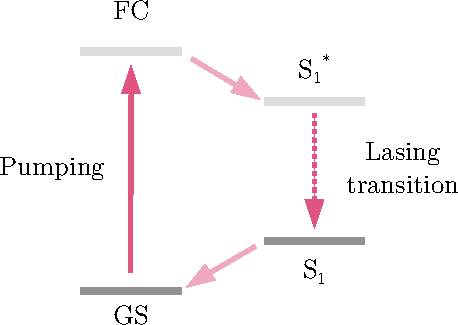
\includegraphics[width=8cm]{Chapters/4Photochem/laser.pdf}
\caption{Diagram of the mechanism behind a four-level laser. Each step in the photocycle is labelled with its usual notation\textemdash{}Ground State (GS), Frank-Condon (FC), excited state minimum (S$_1^*$) and the corresponding ground state (S$_1$).}
\label{fig:laser_diag}
\end{figure}

The four-level structure is motivated by the expression for the Maxwell-Blotzmann thermodynamic equilibrium between two states:
\begin{equation}
    \frac{n_2}{n_1} = e^{-\frac{E_2-E_1}{kT}}
    \label{eq:popinv}
\end{equation}
Where $k$ is the Boltzmann constant, $E_i$ is the energy of state $i$, and $T$ is the temperature. The left-hand side of Equation \ref{eq:popinv} is vanishingly small, indicating that at an equilibrium, $n_1 \gg n_2$. To encourage emission, we should invert this ratio, and take the system out of equilibrium. In our four-level laser example, the 1 state, labelled S$_1$, is very depopulated compared to S$_1^*$ due to the efficient vibrational decay which takes the ground state molecule from its S$_1$ geometry to FC. Thus we have $n_{S_1^*} \gg n_{S_1}$, enabling population inversion.

Additionally, the efficiency of the laser depends on the QEF of the lasing transition. A large Stokes shift is also desirable, to minimise reabsorption, therefore requiring a substantial reorganisation between the FC and S$_1^*$ geometries. Furthermore, if the lasing transition is only accessible through S$_0$\textendash{}S$_1$ absorption, then the S$_1$\textendash{}S$_2$ energy gap should be large enough to discourage absorption to S$_2$ and higher states.

Such specific properties make organic single crystals ideal candidates for laser media. The conformational variety of their crystal packing makes their intermolecular properties tunable, which can principle be exploited to tailor optimal materials. Reference \citenum{Gierschner2016}, reviews a large list of different organic single crystals which desirable emissive properties spanning across the visible spectrum.